% $Header$

\documentclass{beamer}

% This file is a solution template for:

% - Talk at a conference/colloquium.
% - Talk length is about 20min.
% - Style is ornate.



% Copyright 2004 by Till Tantau <tantau@users.sourceforge.net>.
%
% In principle, this file can be redistributed and/or modified under
% the terms of the GNU Public License, version 2.
%
% However, this file is supposed to be a template to be modified
% for your own needs. For this reason, if you use this file as a
% template and not specifically distribute it as part of a another
% package/program, I grant the extra permission to freely copy and
% modify this file as you see fit and even to delete this copyright
% notice. 


\mode<presentation>
{
  %\usetheme{Berkeley}
  %\usetheme{Warsaw}
  \usetheme{CambridgeUS}
  % or ...

  \setbeamercovered{transparent}
  % or whatever (possibly just delete it)
}


\usepackage[english]{babel}
% or whatever

\usepackage[utf8]{inputenc}
% or whatever

\usepackage{times}
%\usepackage[T1]{fontenc}
% Or whatever. Note that the encoding and the font should match. If T1
% does not look nice, try deleting the line with the fontenc.

\usepackage[font=footnotesize,labelformat=empty,
            justification=raggedright,
%            singlelinecheck=false
  ]{caption}
  
\usepackage{upgreek}
  
\title[Graph Cut - 2nd Milestone] % (optional, use only with long paper titles)
{Graph Cut}

\subtitle
{Second Milestone}

\author[Bruno C. Fiss, Max Göttner] % (optional, use only with lots of authors)
{Bruno Coswig Fiss \and Max Göttner}
% - Give the names in the same order as the appear in the paper.
% - Use the \inst{?} command only if the authors have different
%   affiliation.

\institute[TU Berlin] % (optional, but mostly needed)
{
  \inst{1}%
  Institut für Technische Informatik und Mikroelektronik\\
  Technische Universität Berlin}
% - Use the \inst command only if there are several affiliations.
% - Keep it simple, no one is interested in your street address.

\date[\today] % (optional, should be abbreviation of conference name)
{Parallele Algorithmen auf GPUs}
% - Either use conference name or its abbreviation.
% - Not really informative to the audience, more for people (including
%   yourself) who are reading the slides online

\subject{Image processing}
% This is only inserted into the PDF information catalog. Can be left
% out. 



% If you have a file called "university-logo-filename.xxx", where xxx
% is a graphic format that can be processed by latex or pdflatex,
% resp., then you can add a logo as follows:
% graphics stuff

%\usepackage{pgf}
\pgfdeclareimage[interpolate=true,height=1.0cm]{university-logo}{TUBerlin_Logo_rot}
\logo{\pgfuseimage{university-logo}}

\pgfdeclareimage[interpolate=true,height=5.0cm]{formula}{formula}

% (6) the launch timed out and was terminated

% Delete this, if you do not want the table of contents to pop up at
% the beginning of each subsection:
\AtBeginSubsection[]
{
  \begin{frame}<beamer>{Outline}
    \tableofcontents[currentsection,currentsubsection]
  \end{frame}
}


% If you wish to uncover everything in a step-wise fashion, uncomment
% the following command: 

%\beamerdefaultoverlayspecification{<+->}


\begin{document}

\begin{frame}
  \titlepage
\end{frame}

\begin{frame}{Outline}
  \tableofcontents
  % You might wish to add the option [pausesections]
\end{frame}


% Structuring a talk is a difficult task and the following structure
% may not be suitable. Here are some rules that apply for this
% solution: 

% - Exactly two or three sections (other than the summary).
% - At *most* three subsections per section.
% - Talk about 30s to 2min per frame. So there should be between about
%   15 and 30 frames, all told.

% - A conference audience is likely to know very little of what you
%   are going to talk about. So *simplify*!
% - In a 20min talk, getting the main ideas across is hard
%   enough. Leave out details, even if it means being less precise than
%   you think necessary.
% - If you omit details that are vital to the proof/implementation,
%   just say so once. Everybody will be happy with that.

\section{Our Implementation}

\subsection{Recalling Problem...}

\begin{frame}{Using Graph Cut for Energy Minimization}
  % - A title should summarize the slide in an understandable fashion
  %   for anyone how does not follow everything on the slide itself.
   Minimize:
   \begin{figure}
   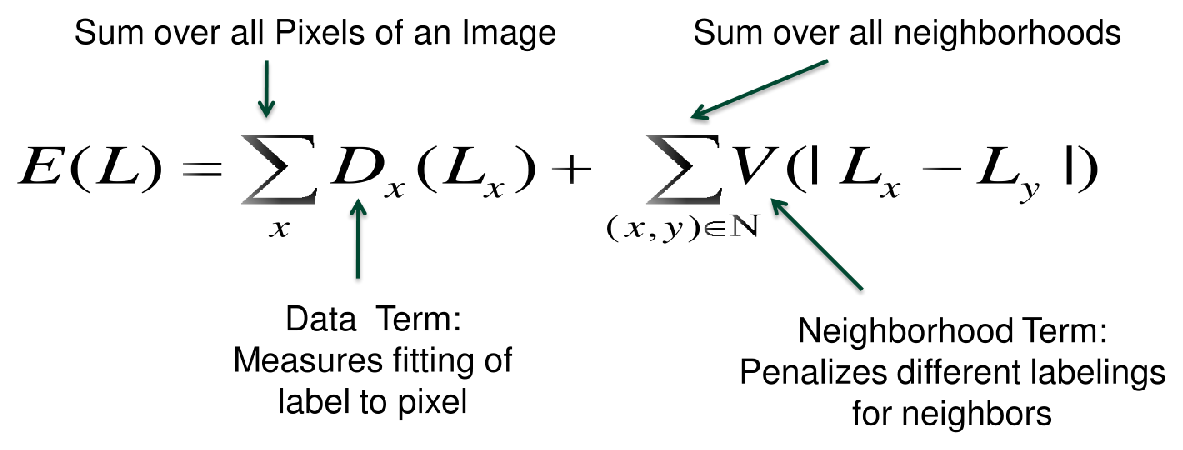
\includegraphics[scale=0.5]{formula} 
   \captionof{figure}{\scriptsize Credit:\thinspace{\small\itshape Timo Stich, 2009}}
   \end{figure}
\end{frame}

\begin{frame}{Using Graph Cut for Energy Minimization}
  % - A title should summarize the slide in an understandable fashion
  %   for anyone how does not follow everything on the slide itself.
   Find minimum cut:
   \begin{figure}
   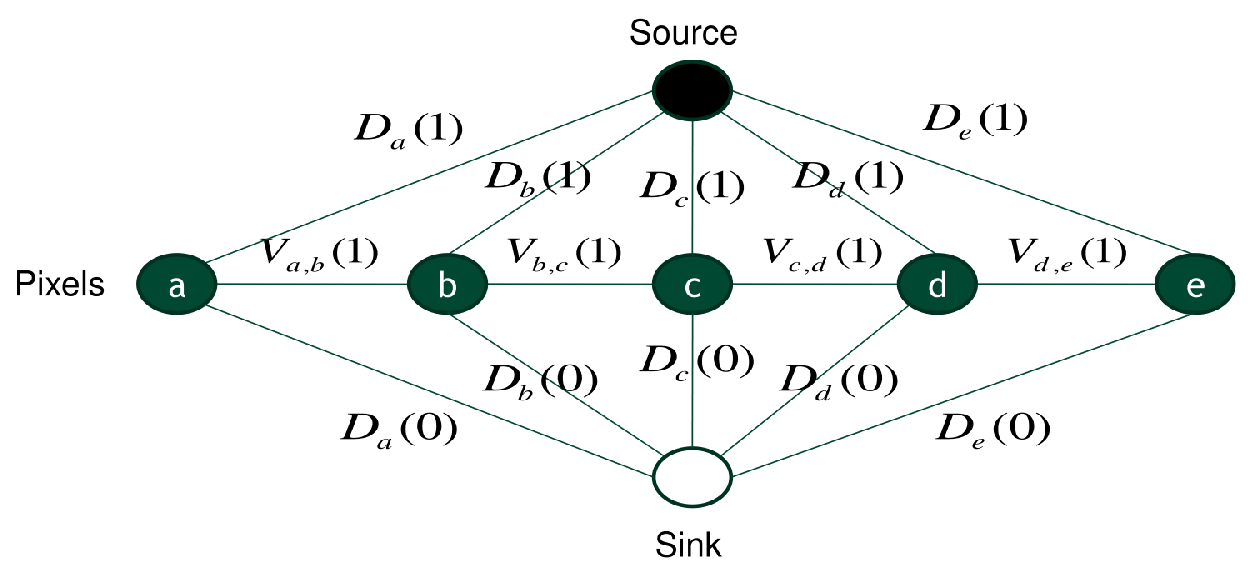
\includegraphics[scale=0.5]{graph} 
   \captionof{figure}{\scriptsize Credit:\thinspace{\small\itshape Timo Stich, 2009}}
   \end{figure}
\end{frame}

\begin{frame}{Using Graph Cut for Energy Minimization}
  % - A title should summarize the slide in an understandable fashion
  %   for anyone how does not follow everything on the slide itself.
   Find minimum cut:
   \begin{figure}
   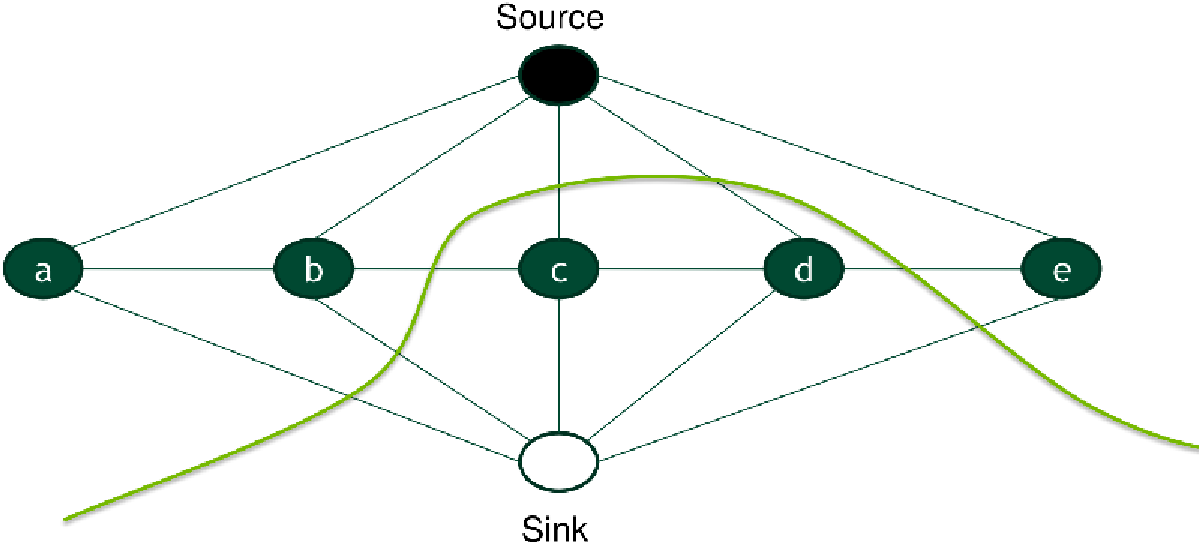
\includegraphics[scale=0.5]{graph2} 
   \captionof{figure}{\scriptsize Credit:\thinspace{\small\itshape Timo Stich, 2009}}
   \end{figure}
\end{frame}

\subsection{Algorithm Overview}

\begin{frame}{Information on Every Node}
	\begin{columns}
	\begin{column}{5cm}
		\begin{figure}
		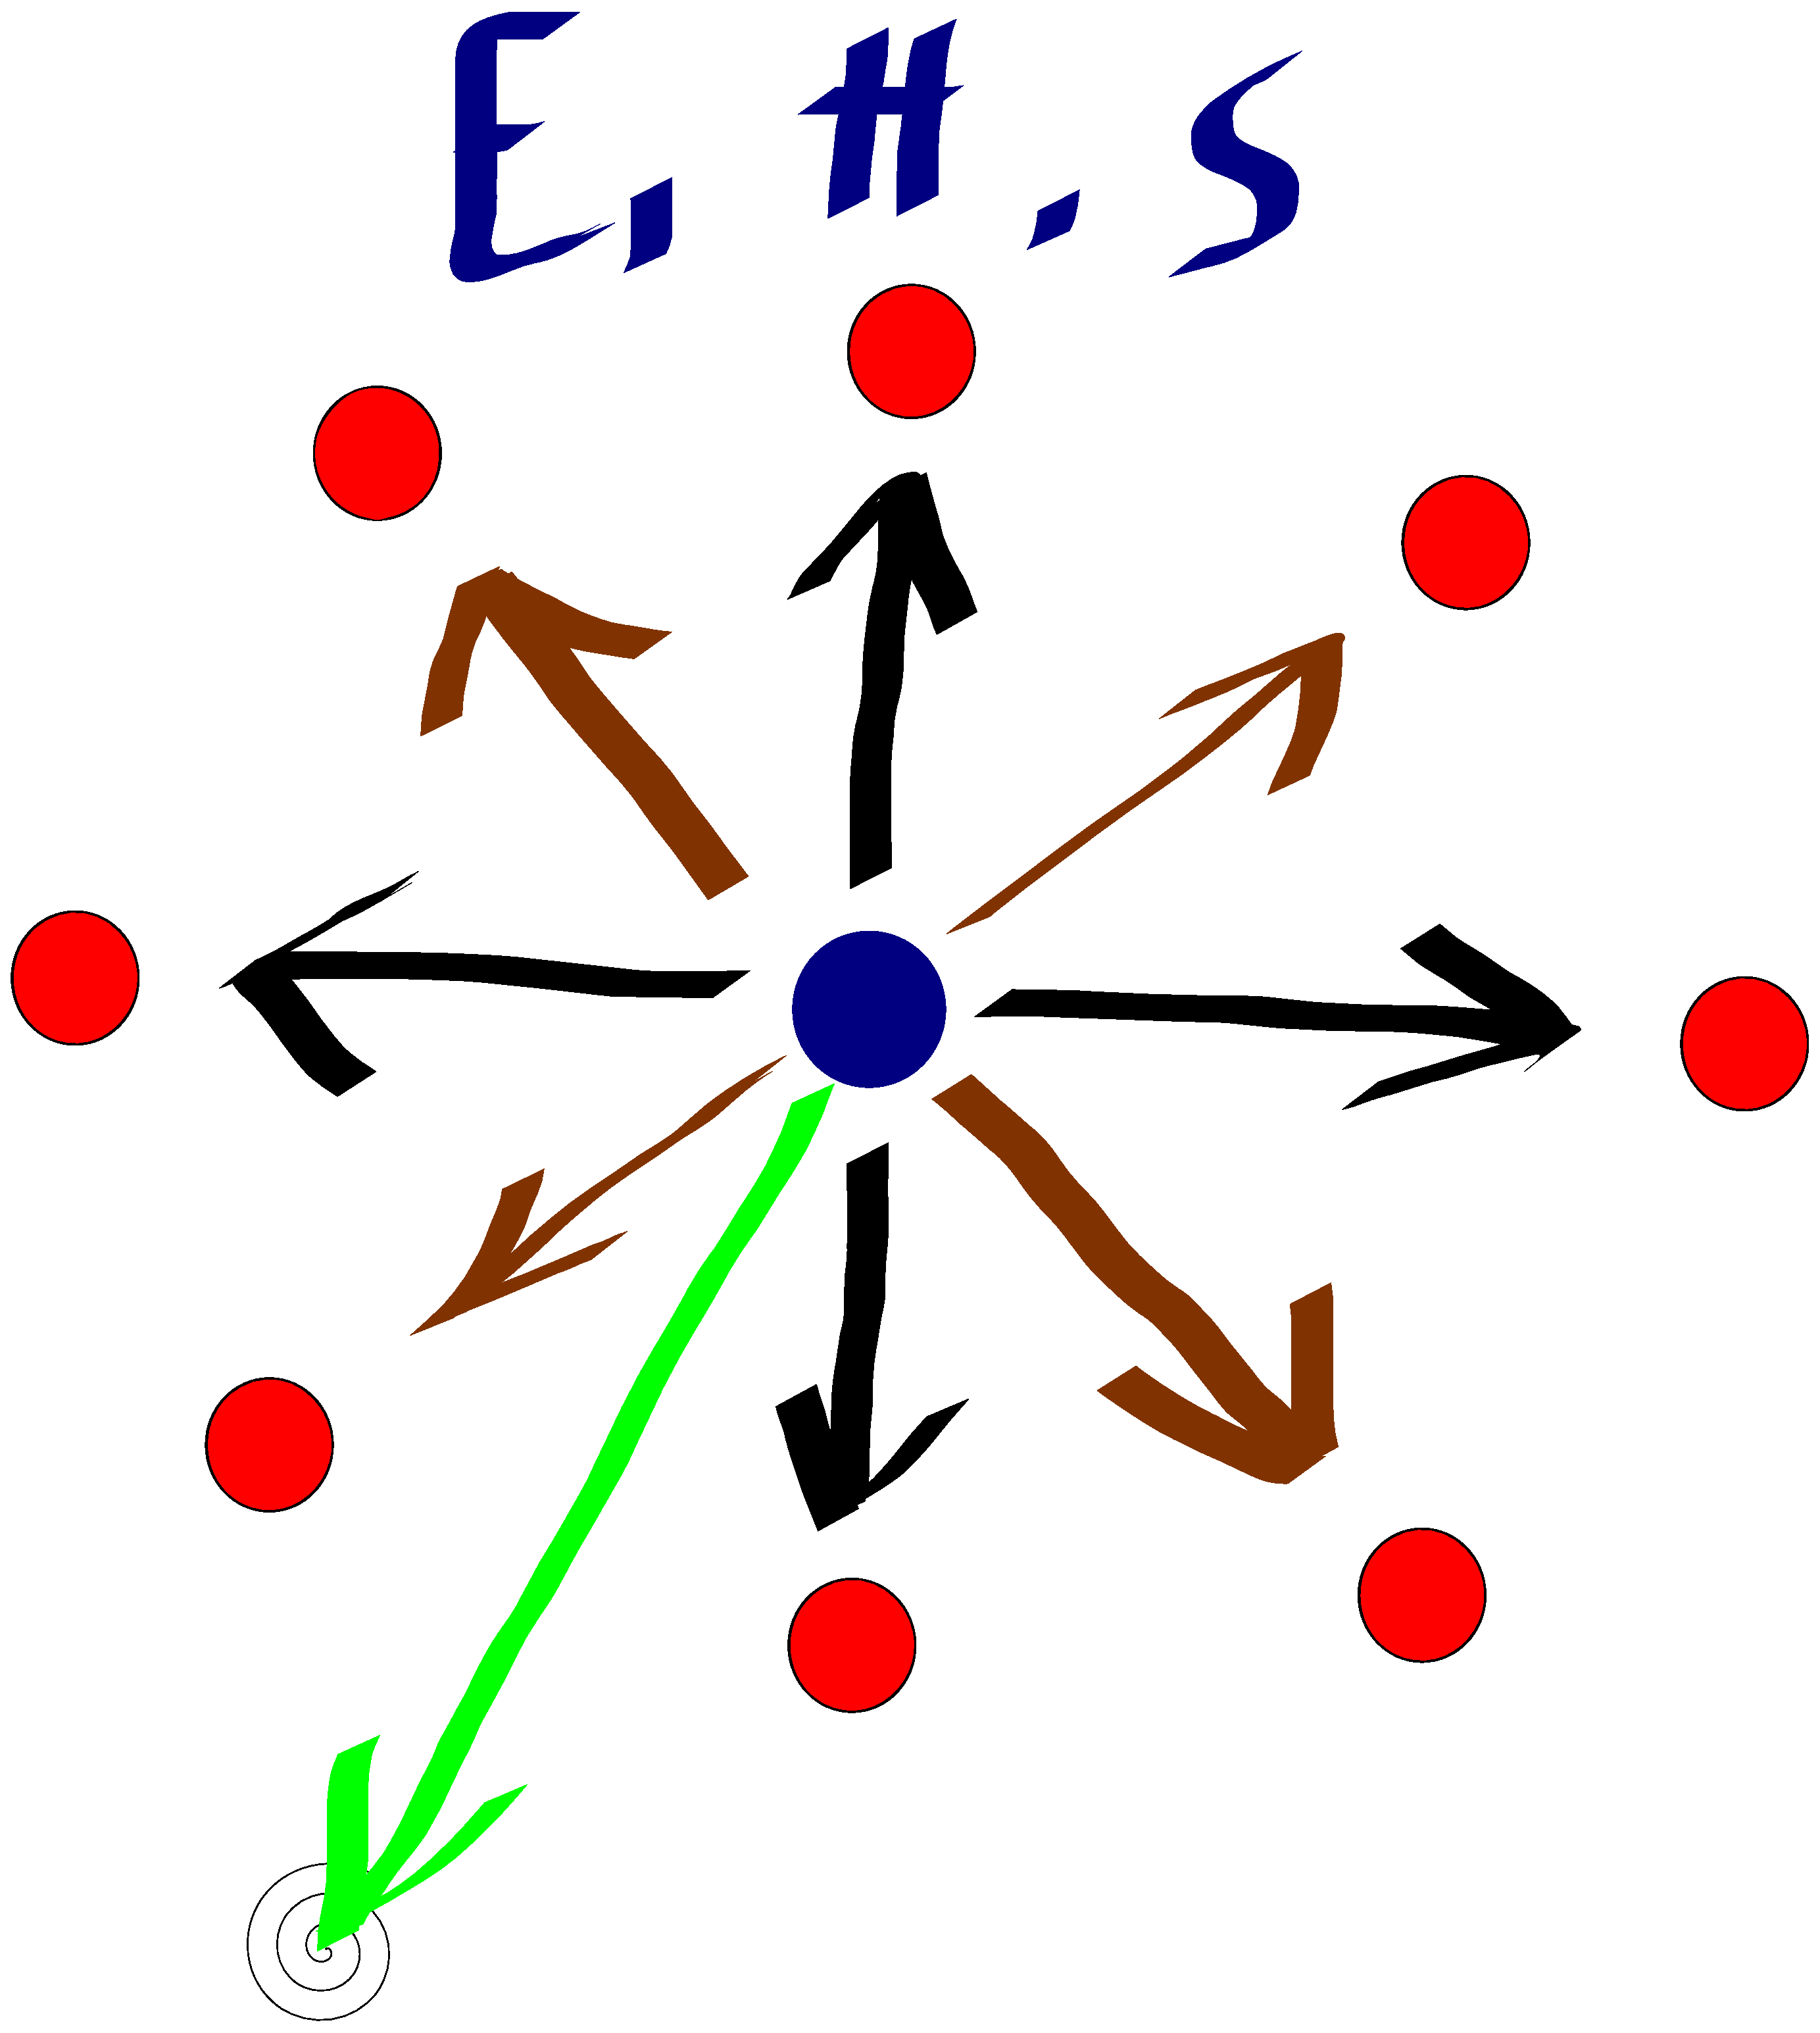
\includegraphics[width=0.9\textwidth]{drawing} 
		%\captionof{figure}{\scriptsize Credit:\thinspace{\small\itshape Timo Stich, 2009}}
		\end{figure}
	\end{column}
	\begin{column}{5cm}
	  Every node has:
	  \begin{itemize}
	    \item
	    Height.
	    \item
	    Excess flow.
	    \item
	    Status (speed-up).
	    \item
	    4-8(!) edges, plus sink.
	  \end{itemize}
	  All are integers.
	\end{column}
	\end{columns}
\end{frame}

\begin{frame}{Implementation Structure}
\begin{itemize}
 \item
 Simple idea: every thread is responsible for one node/pixel.
 \item
 Apply Push and Relabel to every node. Repeat it until flow stops changing.
 \item
 Size blocks appropriately (32x8 threads, based on previous works). Pad if necessary.
 \item
 One kernel to initialize graph.
 \item
 One kernel for Push and another for Relabel.
 \item
 Two kernels to extract labeling.
\end{itemize}
\end{frame}

\begin{frame}{Main Operations}
 Push:
 \begin{itemize}
   \item
   Read the height of all neighbors (\alert{shared memory} applicable).
   \item
   Read/modify excess flow and edge capacities. \\Avoid hazards by using \alert{atomic operations}.
 \end{itemize}
 Relabel:
 \begin{itemize}
   \item
   Read excess flow and edge information. \alert{Boolean} would suffice.
   \item
   Read/modify heights (\alert{shared memory} again applicable).
 \end{itemize}
\end{frame}


\section{Our Results}

\subsection{Skin Detection}

\begin{frame}{Neighborhood Comparison}
      Skin detection based on mixture of Gaussians by Jones, Regh.
		\begin{figure}
		\includegraphics[width=0.5\textwidth]{rihannaO} 
		\captionof{figure}{Original picture (3600x3600).}
		\end{figure}
\end{frame}

\begin{frame}{Neighborhood Comparison}
	\begin{columns}
	\begin{column}{5cm}
		\begin{figure}
		\includegraphics[width=0.9\textwidth]{rihanna} 
		\captionof{figure}{4-Neighborhood, 400 iterations.}
		\end{figure}
	\end{column}
	\begin{column}{5cm}
		\begin{figure}
		\includegraphics[width=0.9\textwidth]{rihanna2} 
		\captionof{figure}{8-Neighborhood, 4000 iterations.}
		\end{figure}
	\end{column}
	\end{columns}
\end{frame}

\begin{frame}{More samples}{Original and Naive}
\begin{columns}
\begin{column}{5cm}
	\begin{figure}
		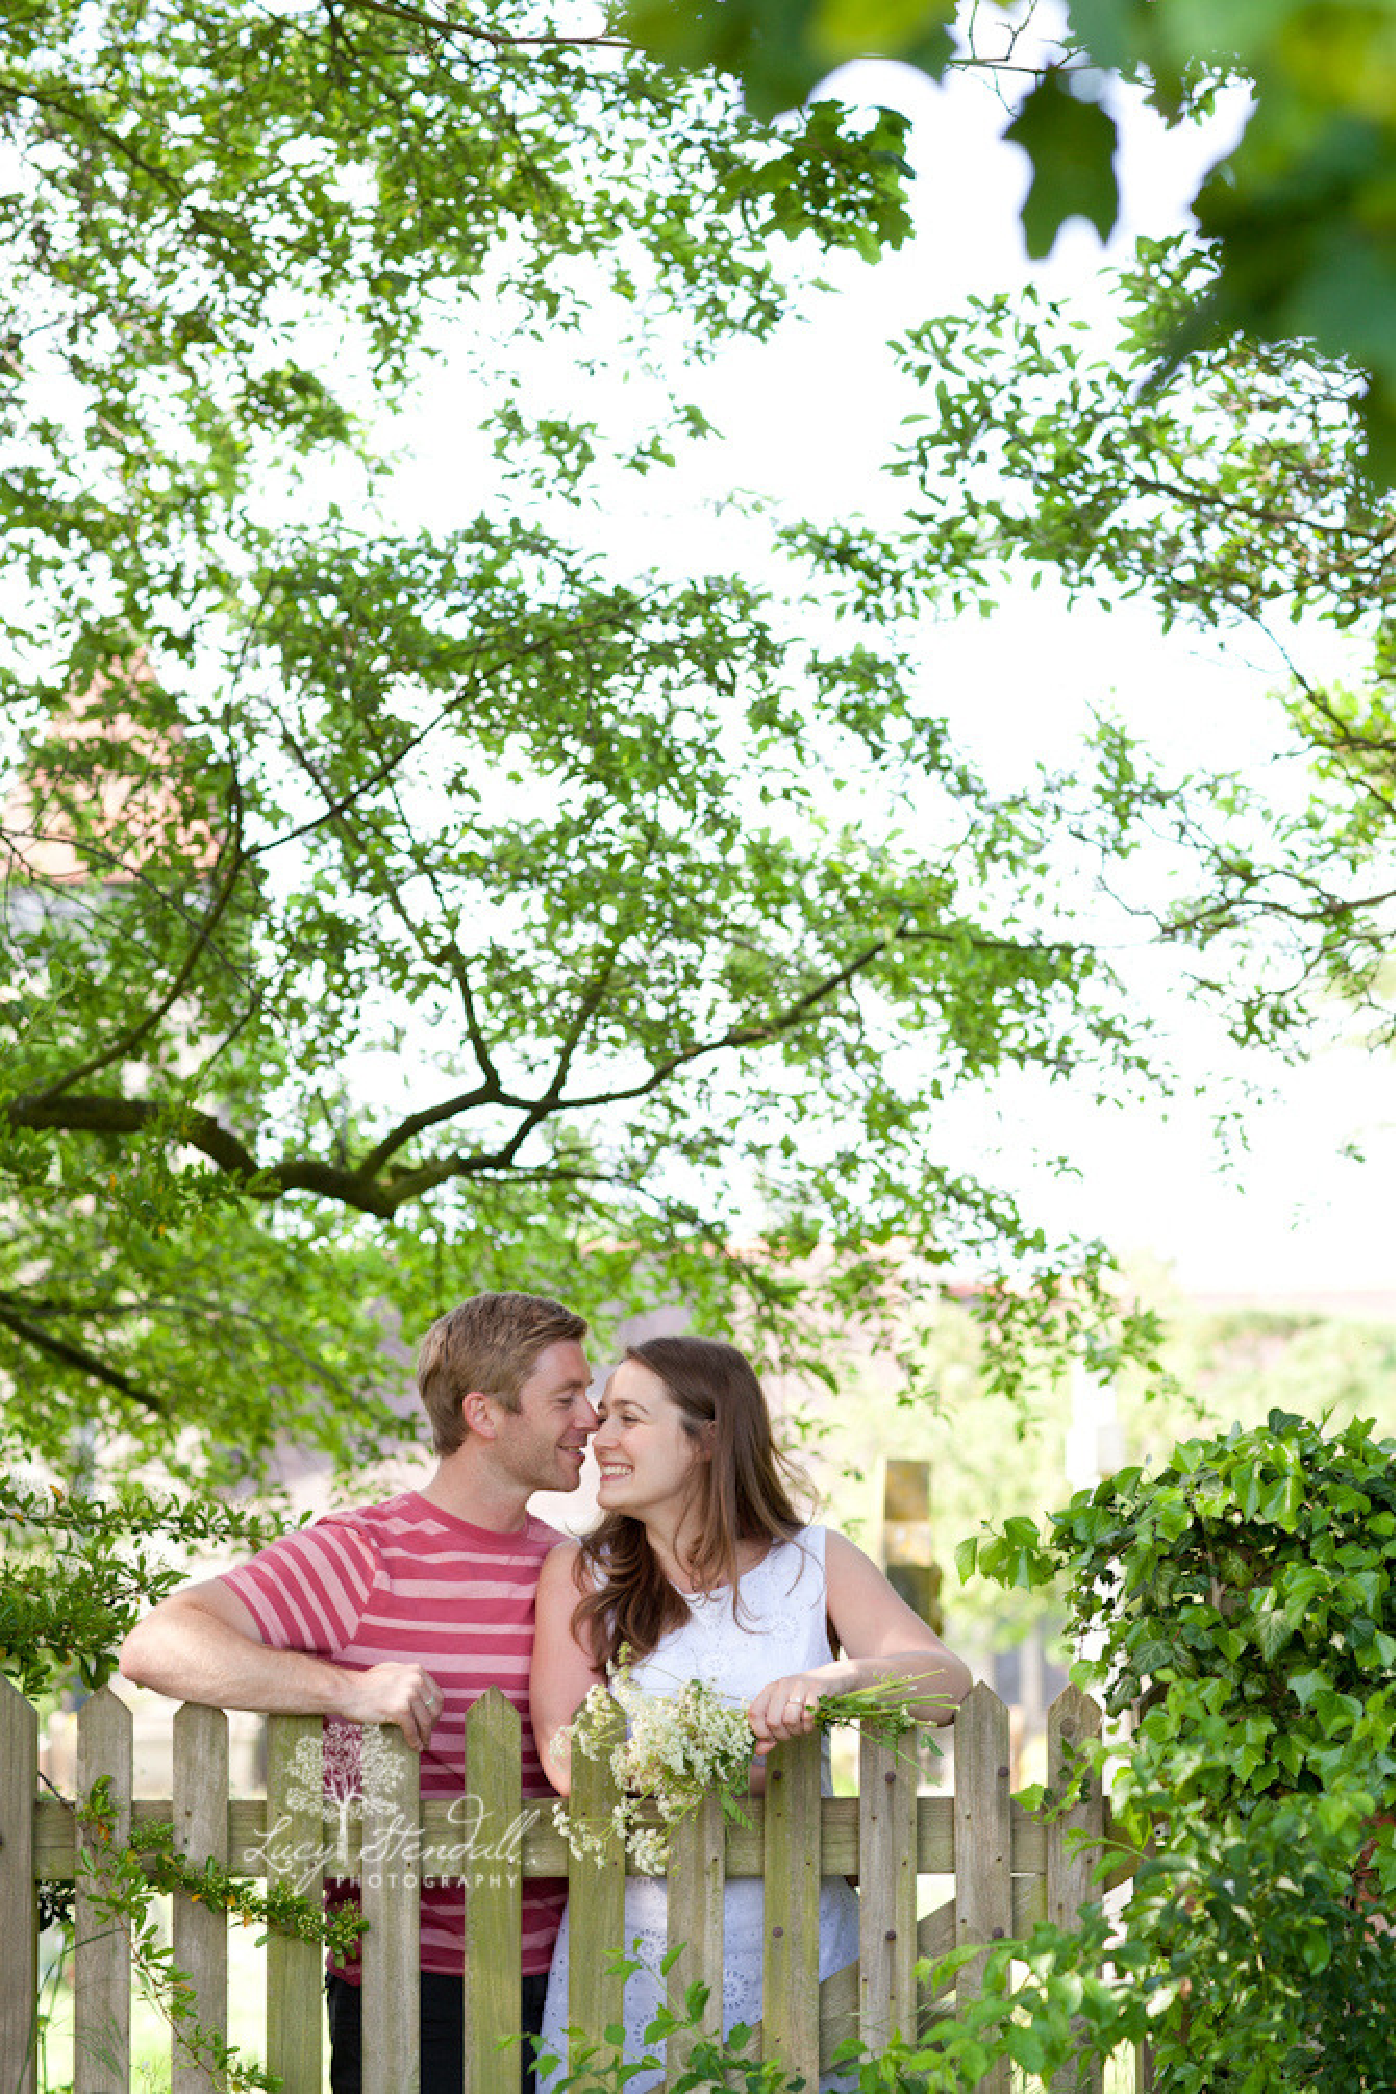
\includegraphics[width=0.8\textwidth]{example} 
		\captionof{figure}{Original picture.}
		\end{figure}
\end{column}
\begin{column}{5cm}
	\begin{figure}
		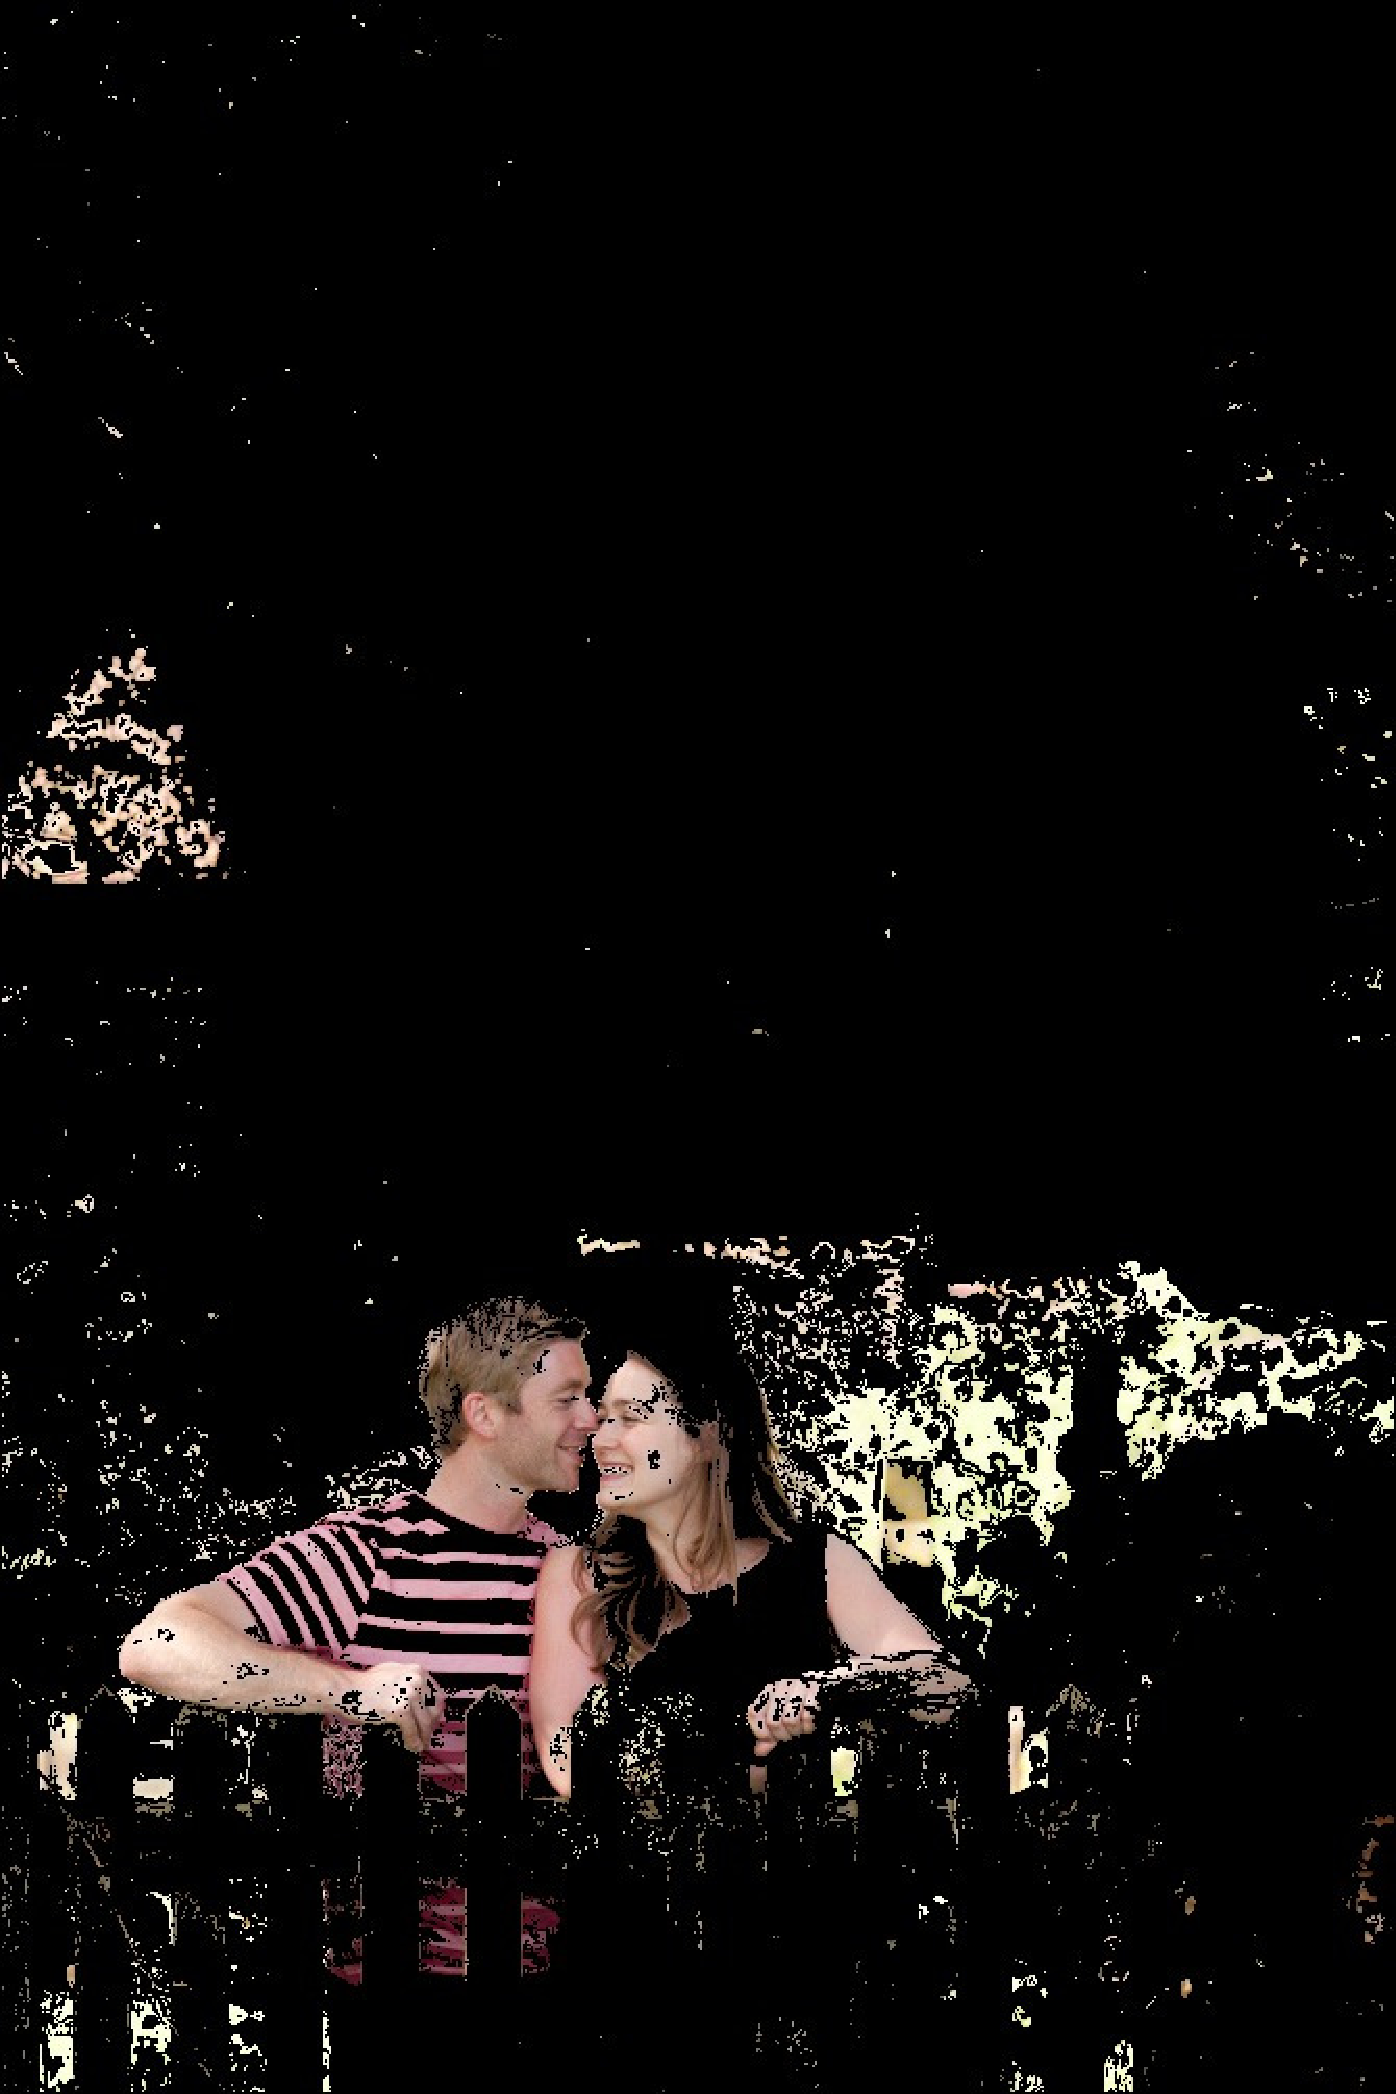
\includegraphics[width=0.8\textwidth]{label0} 
		\captionof{figure}{Naive segmentation.}
		\end{figure}
\end{column}
\end{columns}
\end{frame}

\begin{frame}{More samples}{8-Neighborhood}
\begin{columns}
\begin{column}{3cm}
	\begin{figure}
		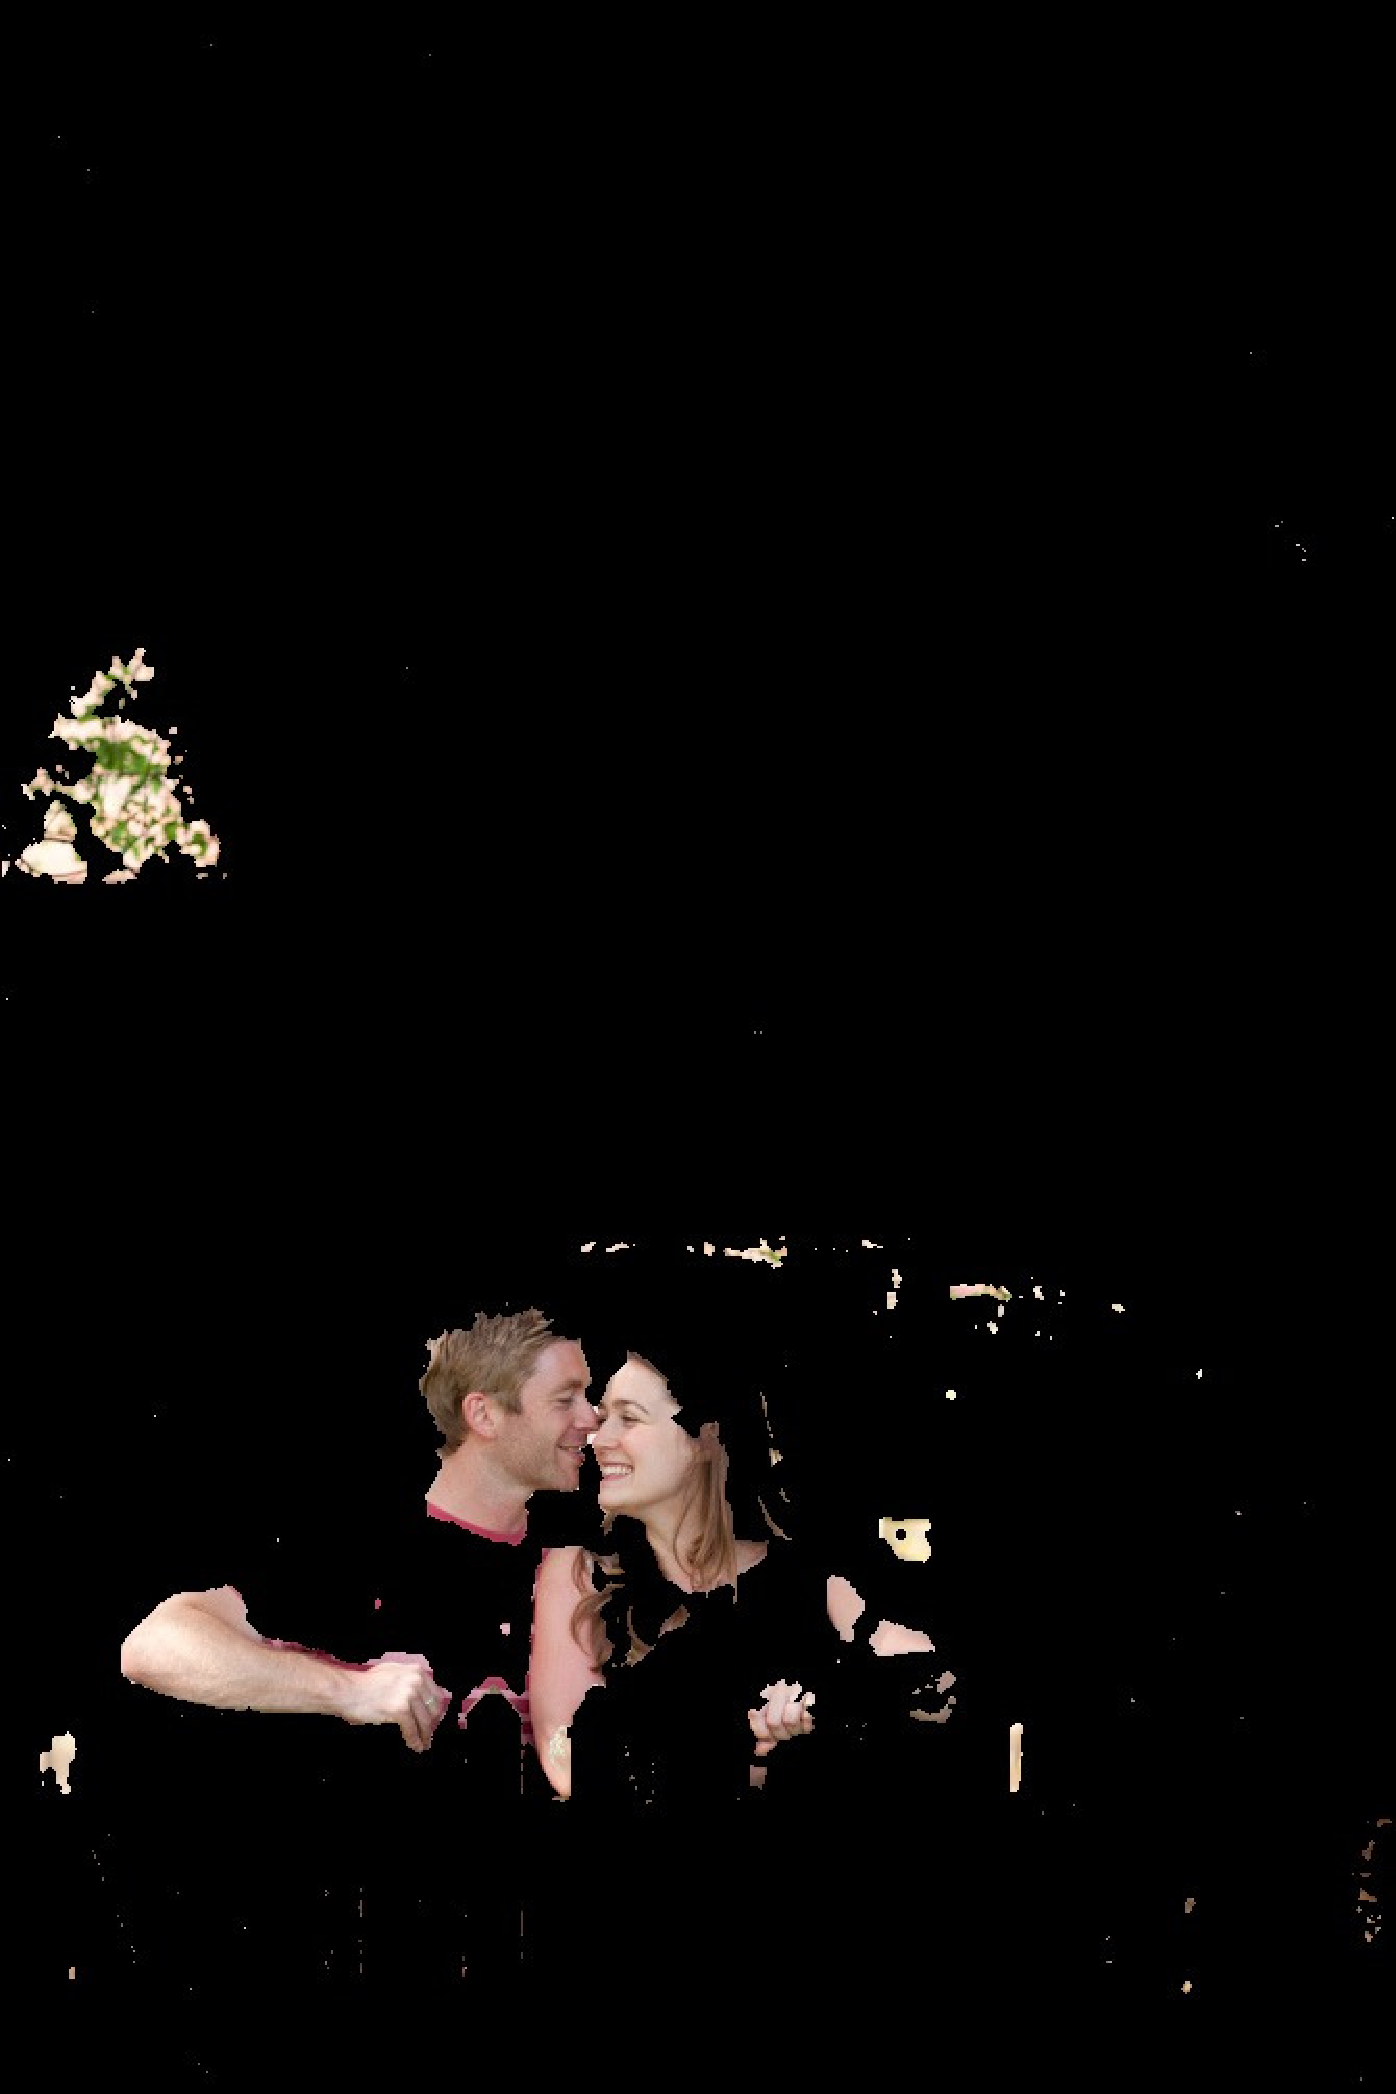
\includegraphics[width=0.9\textwidth]{label1000} 
		\captionof{figure}{Segmentation with P=1000.}
		\end{figure}
\end{column}
\begin{column}{3cm}
	\begin{figure}
		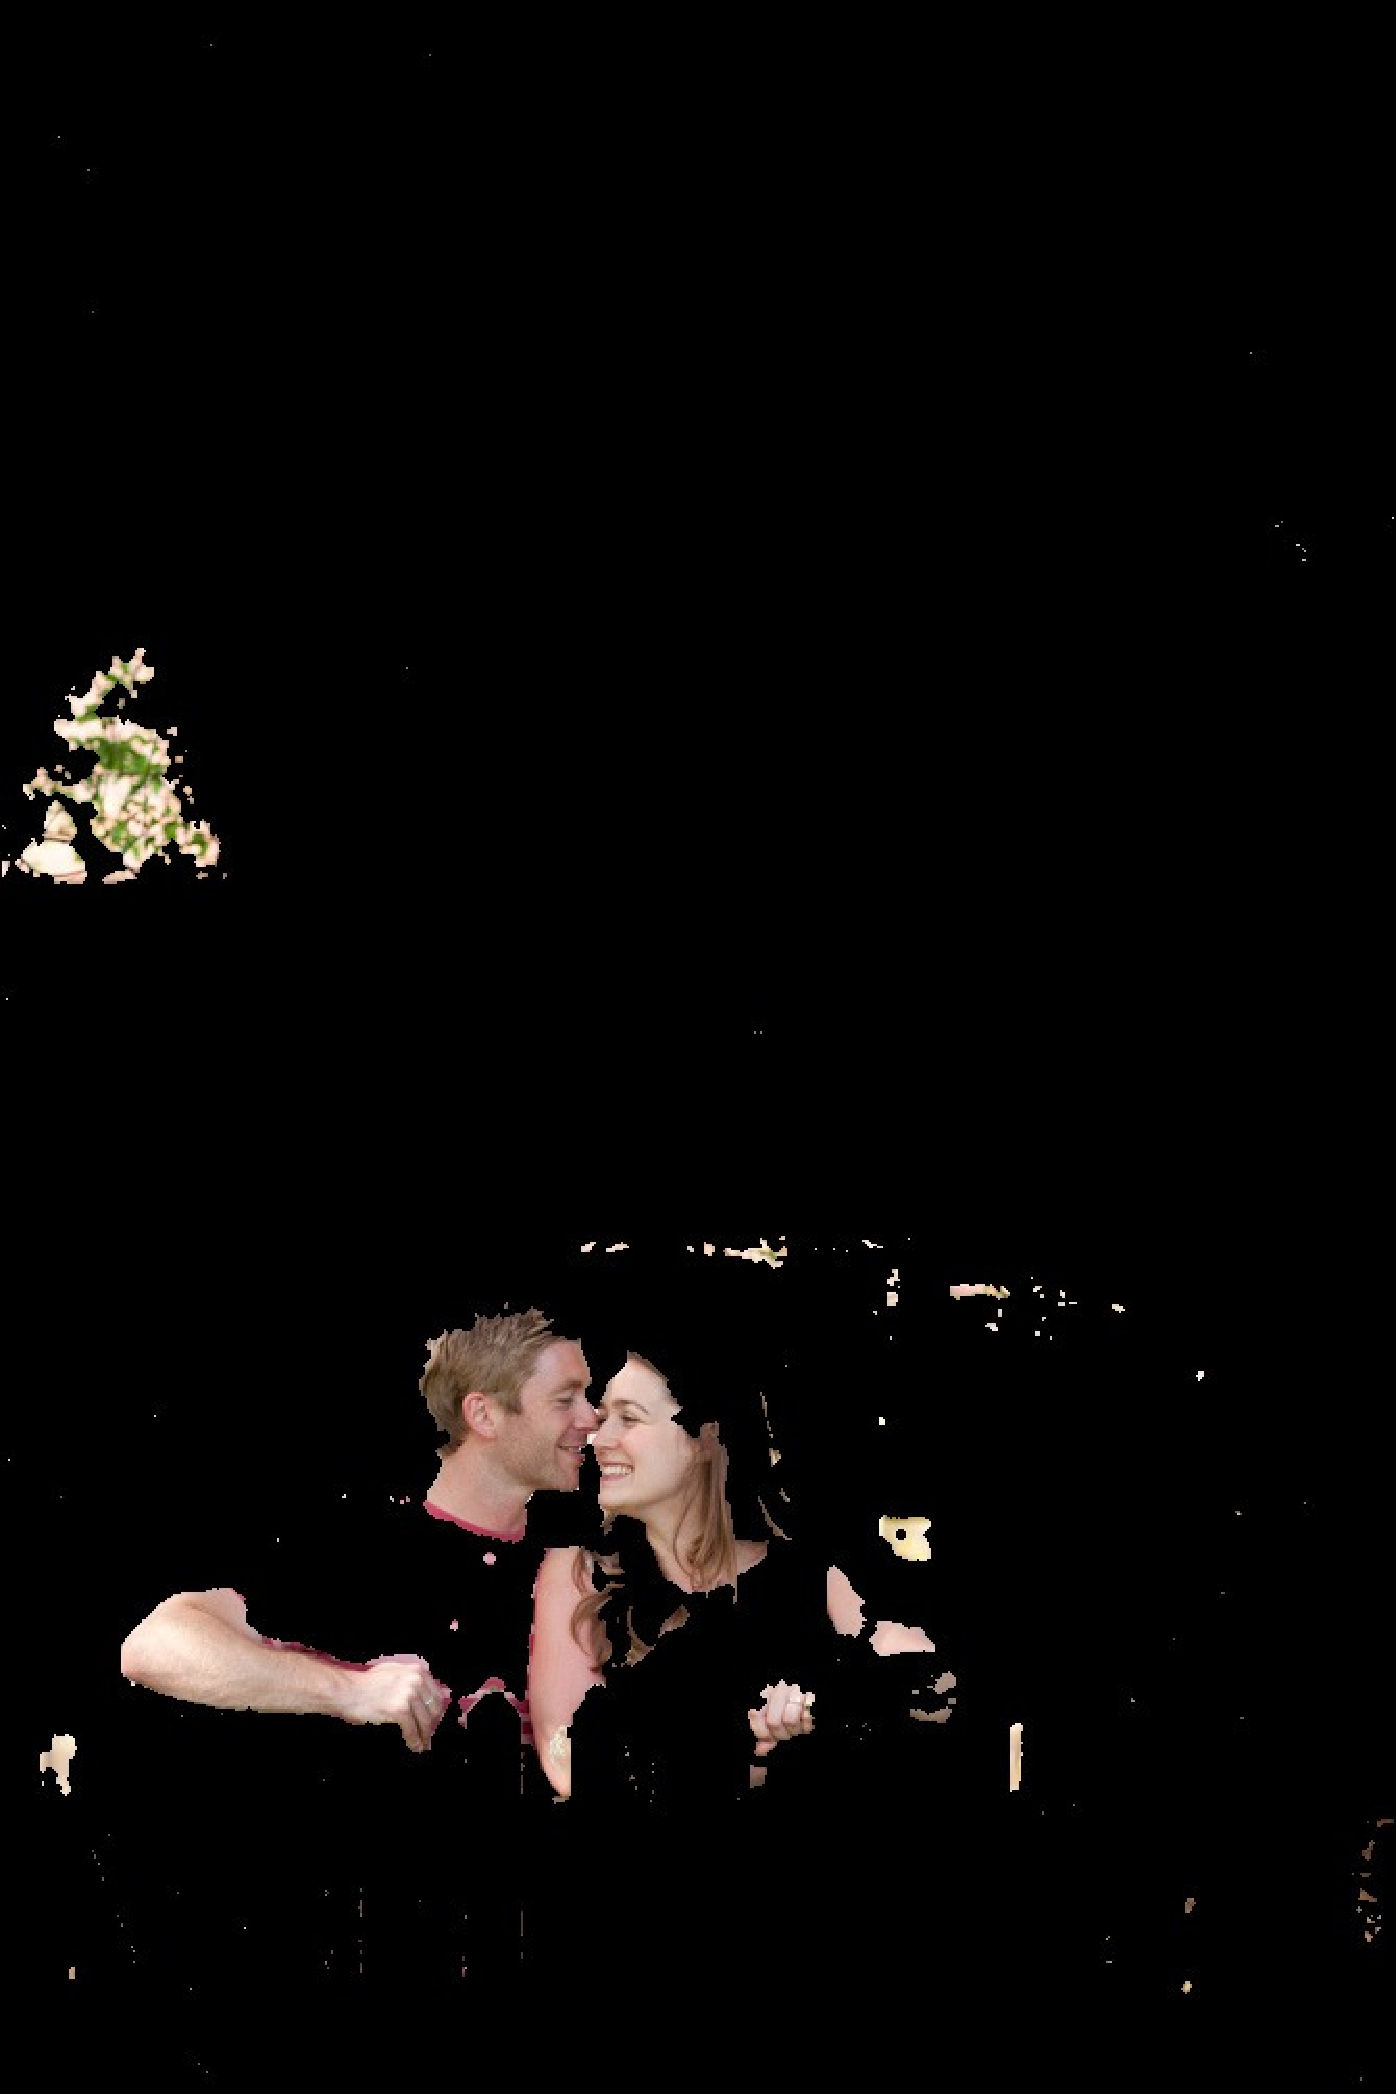
\includegraphics[width=0.9\textwidth]{label1500} 
		\captionof{figure}{Segmentation with P=1500.}
		\end{figure}
\end{column}
\begin{column}{3cm}
	\begin{figure}
		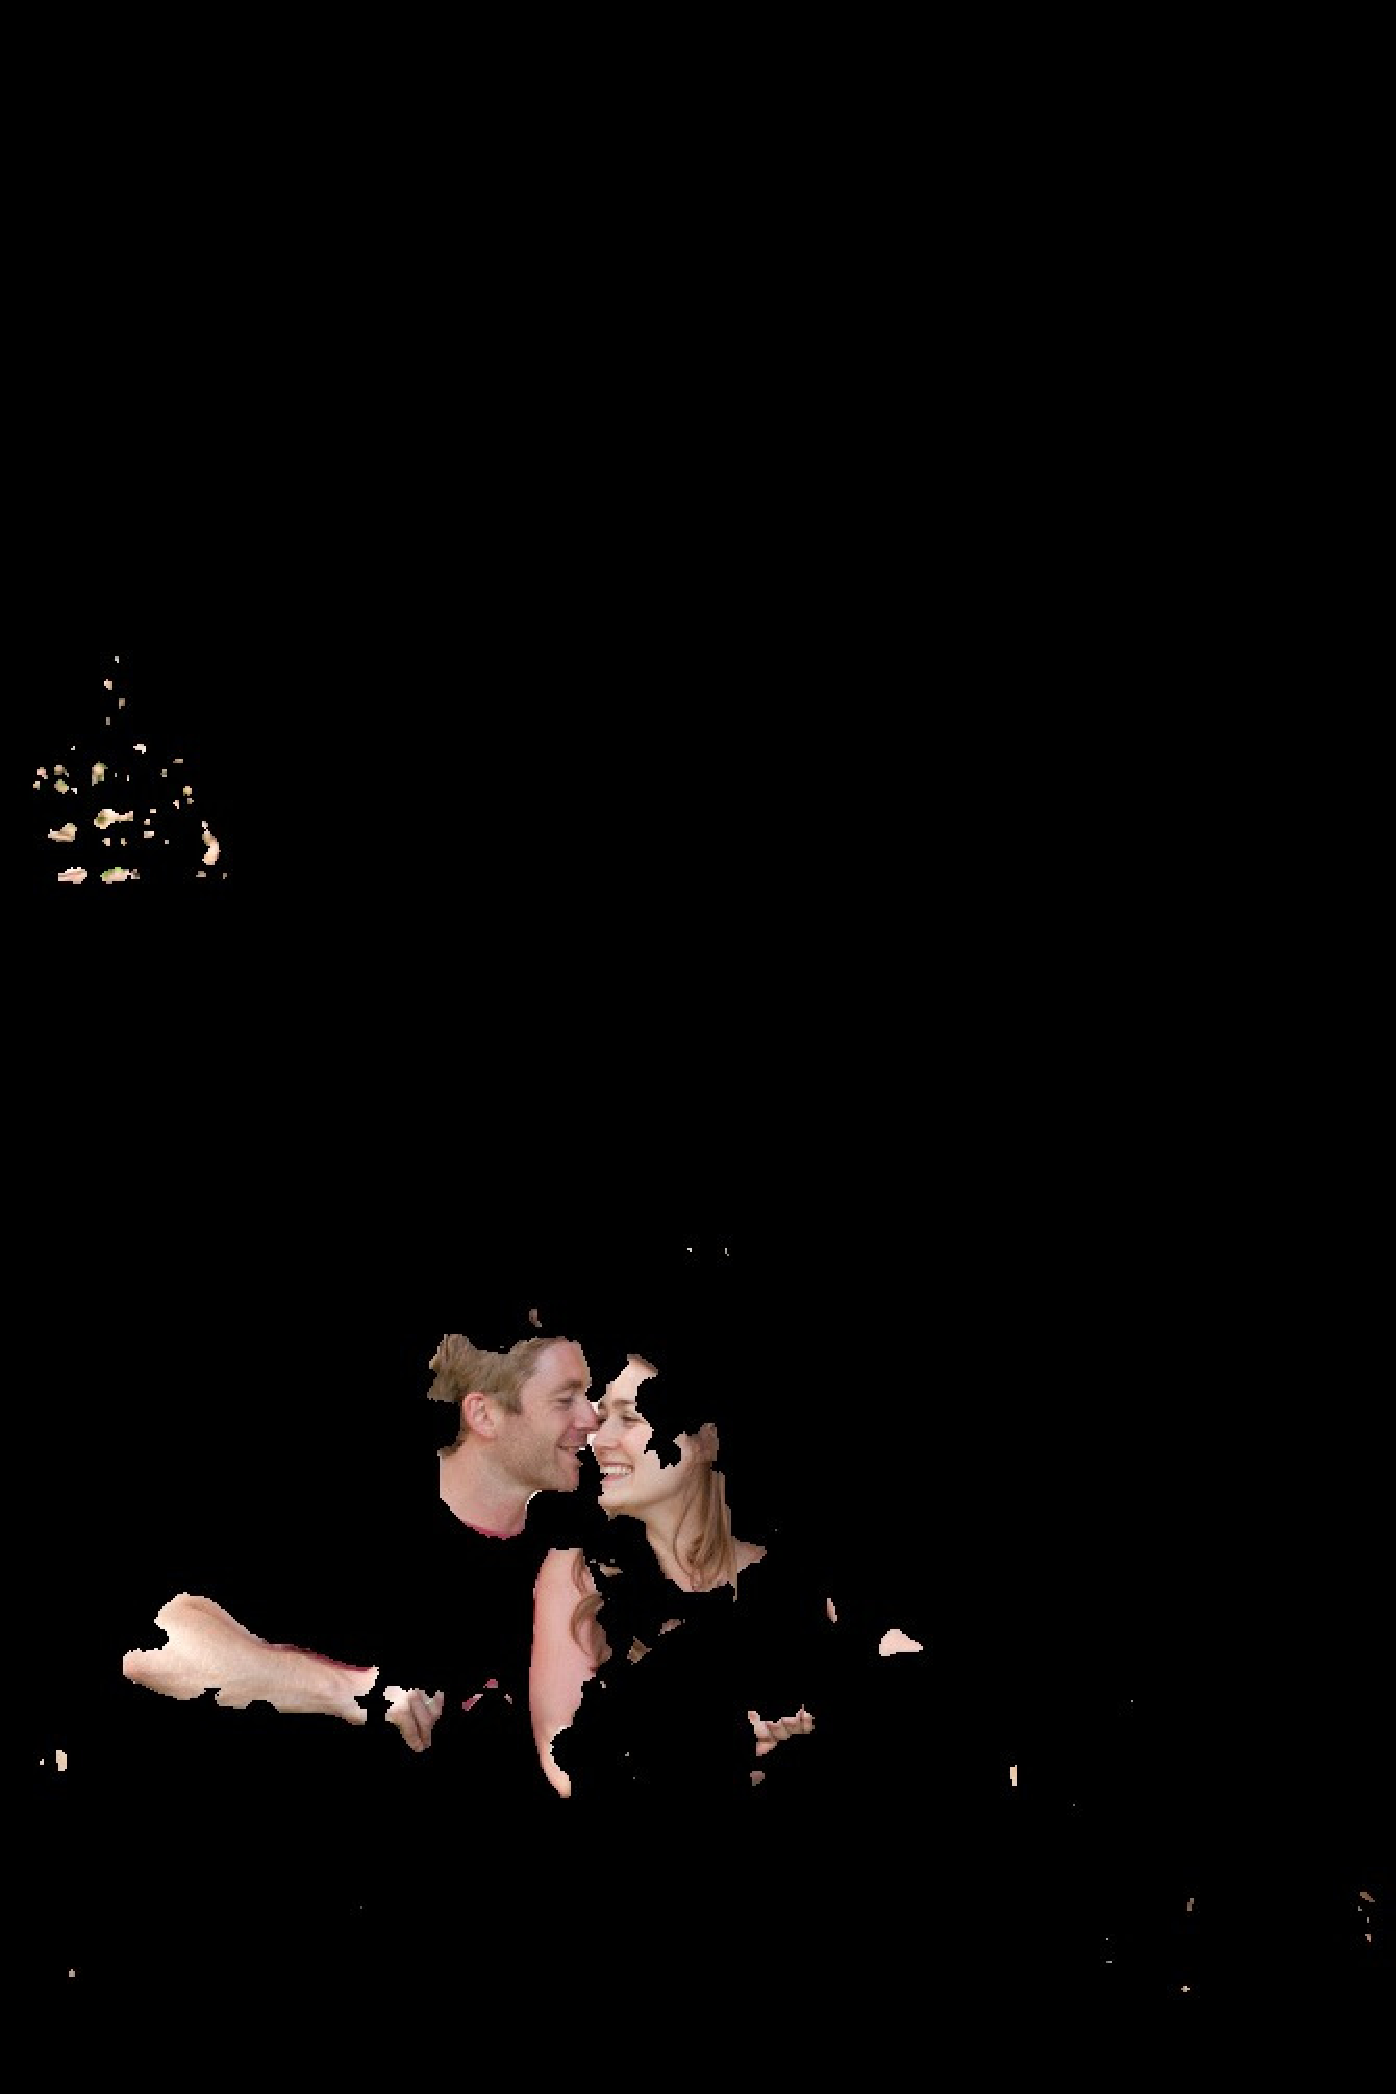
\includegraphics[width=0.9\textwidth]{label2000} 
		\captionof{figure}{Segmentation with P=2000.}
		\end{figure}
\end{column}
\begin{column}{3cm}
	\begin{figure}
		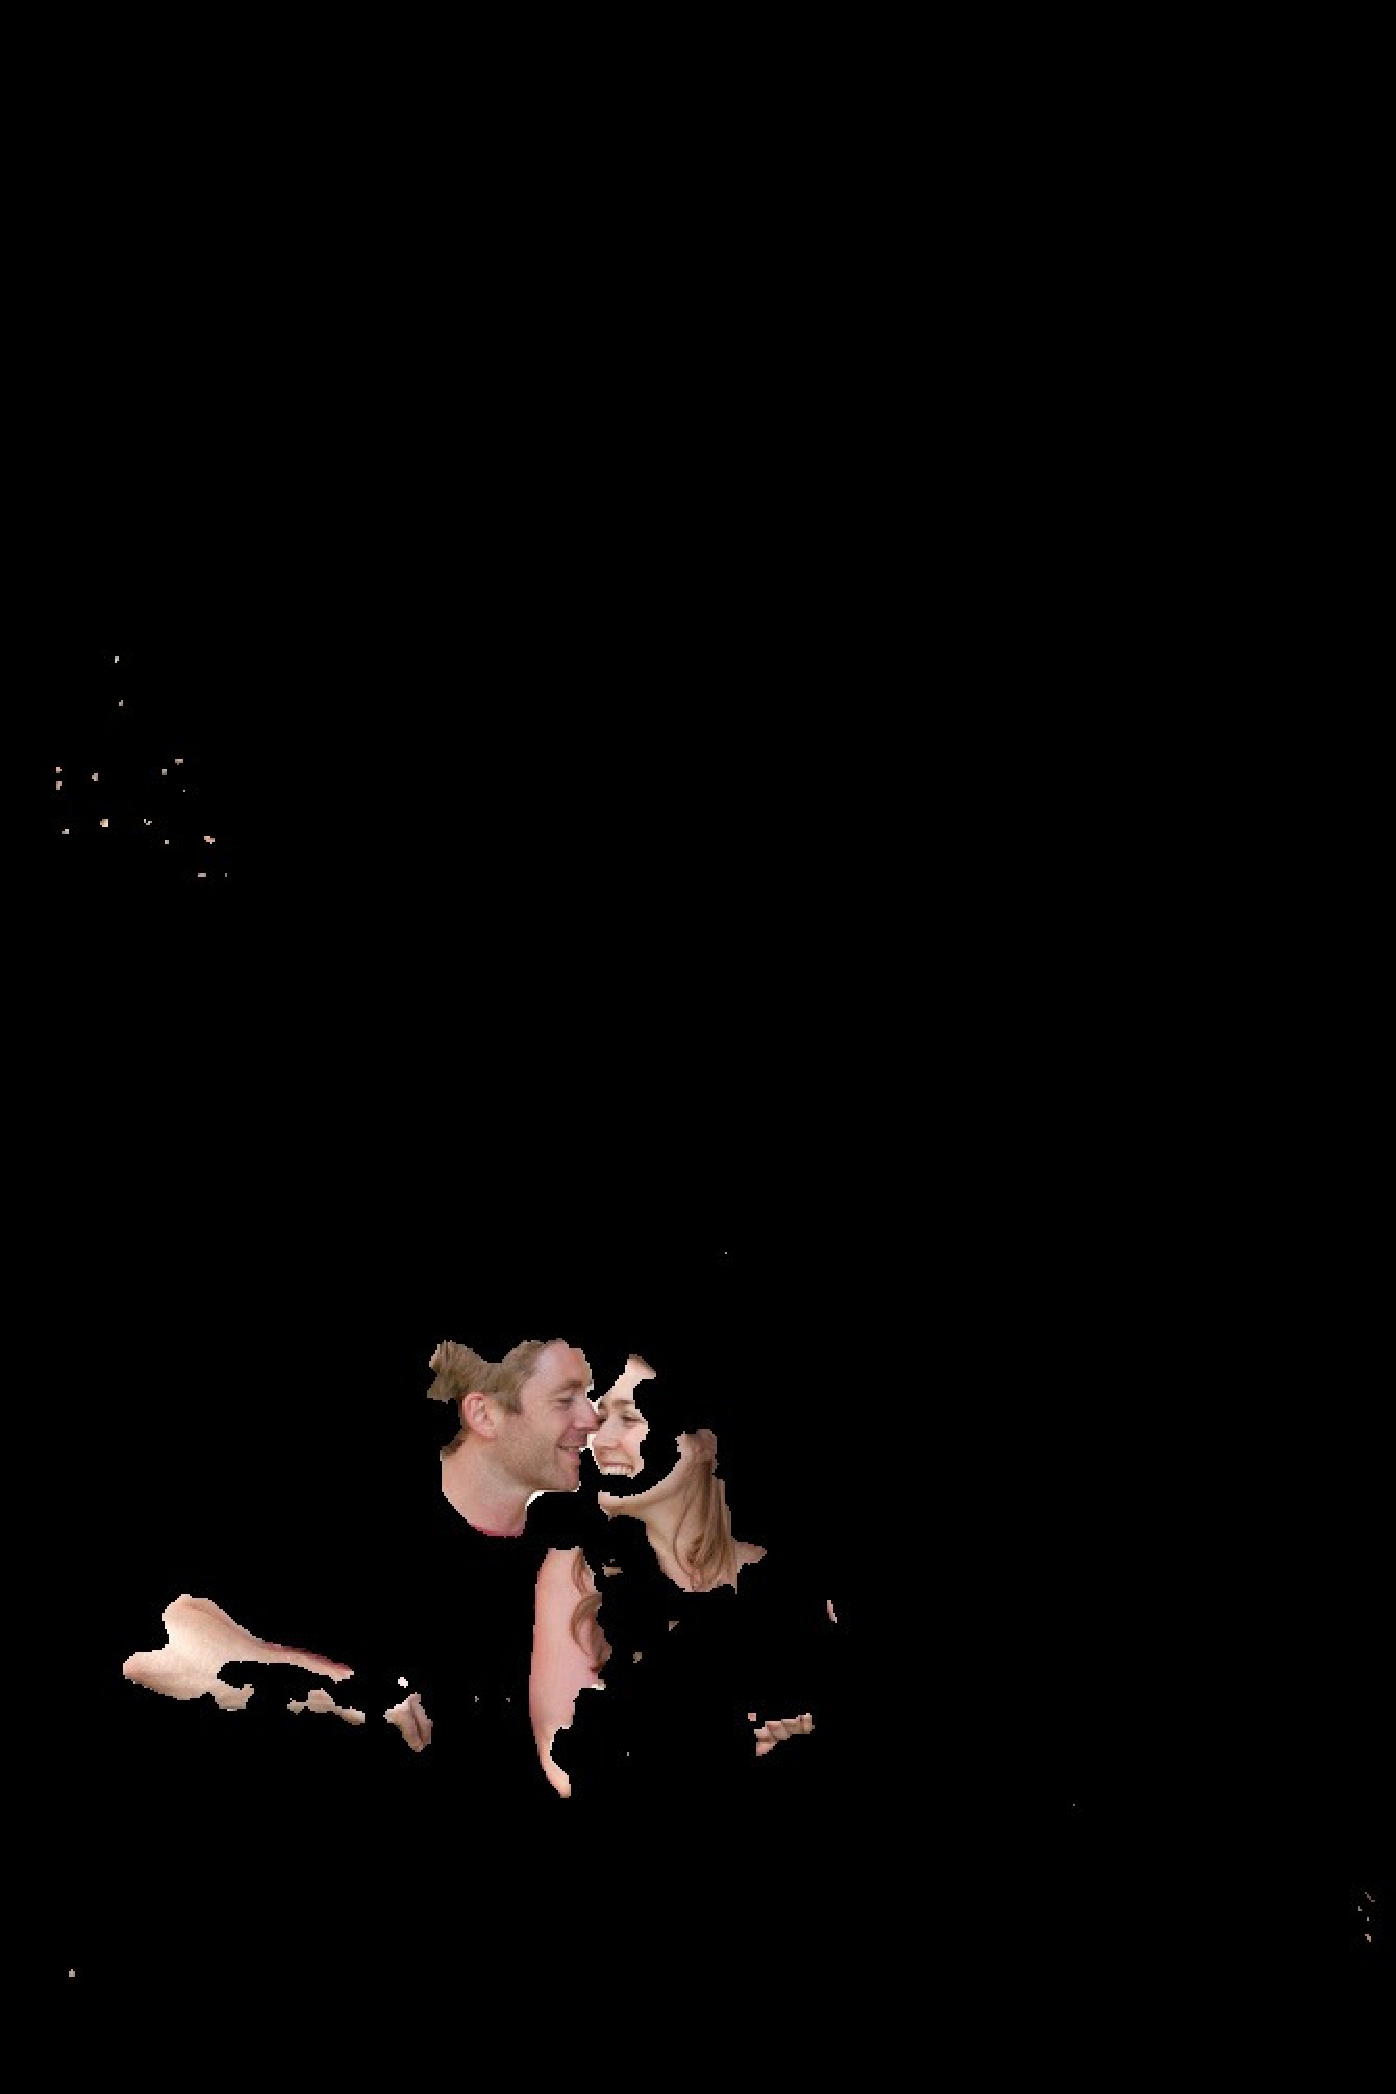
\includegraphics[width=0.9\textwidth]{label2500} 
		\captionof{figure}{Segmentation with P=2500.}
		\end{figure}
\end{column}
\end{columns}
\end{frame}

\subsection{Performance Comparison}

\begin{frame}{Comparison with Previous Works}
Considered works include:
\begin{itemize}
\item
CudaCuts by Vibhav Vineet and P. J. Narayanan, 2008.
\item
Own CPU implementation (for general graphs).
\item
CPU implementation (for specific application) by Boykov \emph{et al.}.
\item
Timo Stich, 2009 (Nvidia \copyright, faster than CudaCuts).
\end{itemize}

 \begin{tabular}{|c|c|}
\hline
\textbf{Implementation} & \textbf{$\mu s$ per iteration} \\
\hline
CudaCuts (640x480) &  122.23 \\
Ours with 8-N (640x480) &  101.10  \\
Ours with 4-N (640x480) &  71.01  \\
Ours with 4-N (3600x3600) &  5319.82  \\
\hline
\end{tabular}
\end{frame}

\begin{frame}{Further Comparison with Previous Works}
\begin{itemize}
\item
Currently only per iteration comparisons done.
\item
CPU implementations and GPU without source are not yet comparable.
\item
For a broader comparison, equal test cases must be used.
\item
Our number of iterations is still high(!): \alert{Global Relabeling} technique necessary.
\end{itemize}
\end{frame}

\section{Next Steps}

\subsection{Performance Improvement}

\begin{frame}{List of Performance Improvements}
\begin{itemize}
\item
Use shared memory for accessing heights (done).
\item
Keep list of active and inactive blocks (done, can be improved).
\item
Use Global Relabeling (currently ``manually'').
\item
Height double buffering (because of memory boundness).
\item
Compress neighbor and edge status.
\item
Use Wave Push (and Wave Global Relabel).
\item
Use Dynamic Updating.
\end{itemize}
\end{frame}

\subsection{Problems}

\begin{frame}{List of Problems}
\begin{itemize}
\item
The implementation depends on atomic functions (sm\_11).
\item
Too many atomic accesses(?) end up generating: (6) the launch timed out and was terminated. [GPU also in use for display]
\item
Both can be solved by using the \alert{Wave technique}.
\end{itemize}
\end{frame}

\subsection{Other Applications}

\begin{frame}{Finding More Applications}
\begin{columns}
\begin{column}{4cm}
   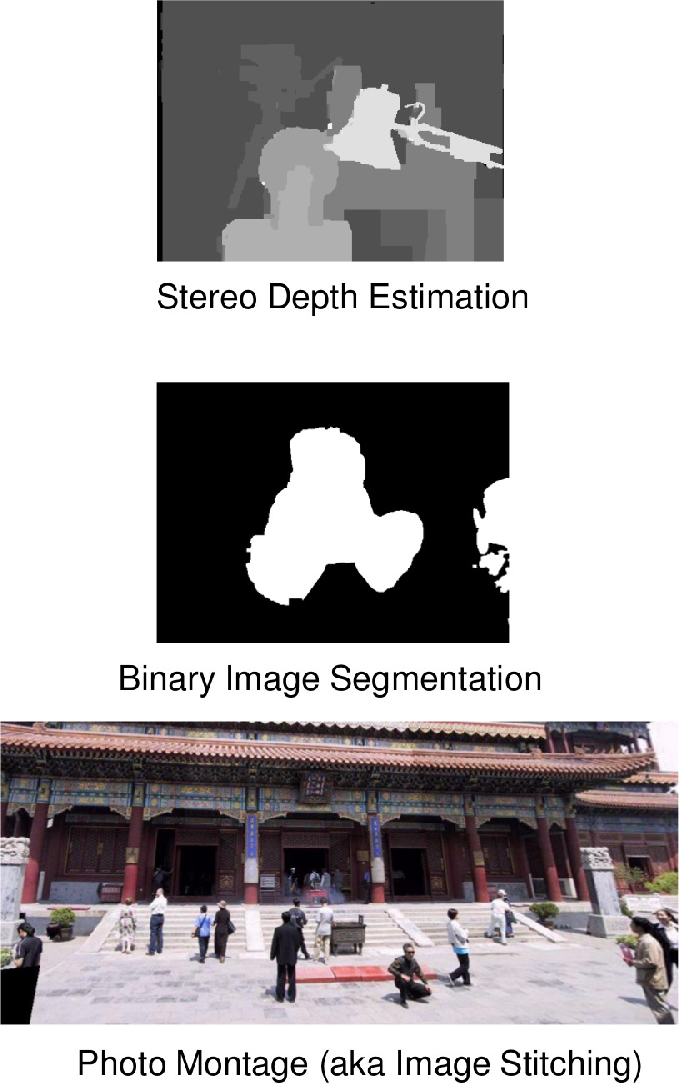
\includegraphics[width=1.0\textwidth]{apps} 
   \captionof{figure}{\scriptsize Credit: MRF Evaluation, Middlebury College}
\end{column}
\begin{column}{6cm}
\begin{itemize}
\item
Skin detection (done - {\raise.17ex\hbox{$\scriptstyle\mathtt{\sim}$}}40ms per 800x600 frame).
\item
Segmentation background/foreground.
\item
Image Stitching.
\item
Stereo Depth Estimation.
\end{itemize}
\end{column}
\end{columns}
\end{frame}

% http://cvit.iiit.ac.in/papers/rtGCuts_2008.pdf
% http://www.nvidia.com/content/GTC/documents/1060_GTC09.pdf
% http://vision.middlebury.edu/

\section*{Thank you!}

\begin{frame}{Conclusion}

  % Keep the summary *very short*.
  \begin{itemize}
  \item
    Suggestions or questions?
  \item
    \alert{Thank you!}
  \end{itemize}
  
  % The following outlook is optional.
  \vskip0pt plus.5fill
  \begin{itemize}
  \item
    Some additional material and references:
    \begin{itemize}
    \item
      \url{http://cvit.iiit.ac.in/papers/rtGCuts_2008.pdf}
    \item
      \url{http://www.nvidia.com/content/GTC/documents/1060_GTC09.pdf}
    \item
      \url{http://vision.middlebury.edu/}
    \end{itemize}
  \end{itemize}
\end{frame}


\end{document}


